\subsubsection{Tent map (TENT)} \label{sssec:tent}

The Tent map has been extensively studied in the literature because theoretically it has nice  statistical properties that can be analytically obtained. For example it is easy to proof that it has a uniform histogram and consequently an ideal $H_{val}=1$. The Perron-Frobenius operator and its corresponding eigenvalues and eigenfunctions may be also be analytically obtained for this map \cite{tent}. 

This map is represented with the equation:
\begin{equation}\label{eq:tentmap}
x_{n+1}~=~ \left\{ \begin{array}{ll}
2~{x_n} & \textrm{if ~$0\leq x_n\leq 1/2$}\\
2~(1-{x_n}) & \textrm{if ~$1/2<x_n\leq 1$} 
\end{array} \right.  \ ,
\end{equation}
with $x_n\in\mathcal{R}$.

In Base-2 fractional numbers rounding, equation \ref{eq:tentmap} became
\begin{equation}\label{eq:tentdecbin}
x_{n+1}~=~ \left\{ \begin{array}{ll}
2~{x_n} & \textrm{if $0\leq x_n\leq 1/2$}\\
\epsilon \times floor\{\frac{2~-~2~x_n}{\epsilon}\} & \textrm{if $1/2<x_n\leq 1$} 
\end{array} \right.  \ ,
\end{equation}
with $\epsilon=2^{-B}$ for binary numbers.

When this map is implemented in a computer using any numerical representation system (even floating point!) truncation errors rapidly increases and makes the unstable fixed point in $x^*=0$ becomes stable producing a short transitory of length between $0$ and $B$ followed by an infinite number of  $0$'s \cite{Jessa1993,Callegari1997}.
This issue is easily explained in [with chaos meet computers], problem appears because all itarations has an shift-to-left operation that carry the $0$'s from the right side of the number.
Some authors \cite{buscar} have proposed to add a random perturbation to avoid this drawback of the Tent map. But this procedure introduces statistical properties of the random perturbation that are mixed with those of the Tent map itself.
Skew Tent is an option that allows reach nice statistical properties even in base 2 fractional numbers.
Here we study the Tent map "as it is" without any artifact to evaluate its real instead of theoretical statistical properties. 

Figs. \ref{fig:TENT_QuantiB} (a) to (e) shows the quantifiers for floating and fixed point numerical representation.
Quantifiers $H_{val}$, $H_{BP}$ and $C_{BP}$ are equal to zero for all presitions, this reflects that the series remains in a fixed point for almost all samples. 
When we compares with $H_{BPW}$ and $C_{BPW}$ quantifiers they are different of $0$ because $BPW$ procedure discards the elements once they reach the fixed point.
High dispersions in $H_{BPW}$, $C_{BPW}$ and $MP$ are related with the short length of data taken into account, transient to fixed point has a maximum length of $B$ iterations for fixed point arithmetic and $54$ for floating point.

\begin{figure}
	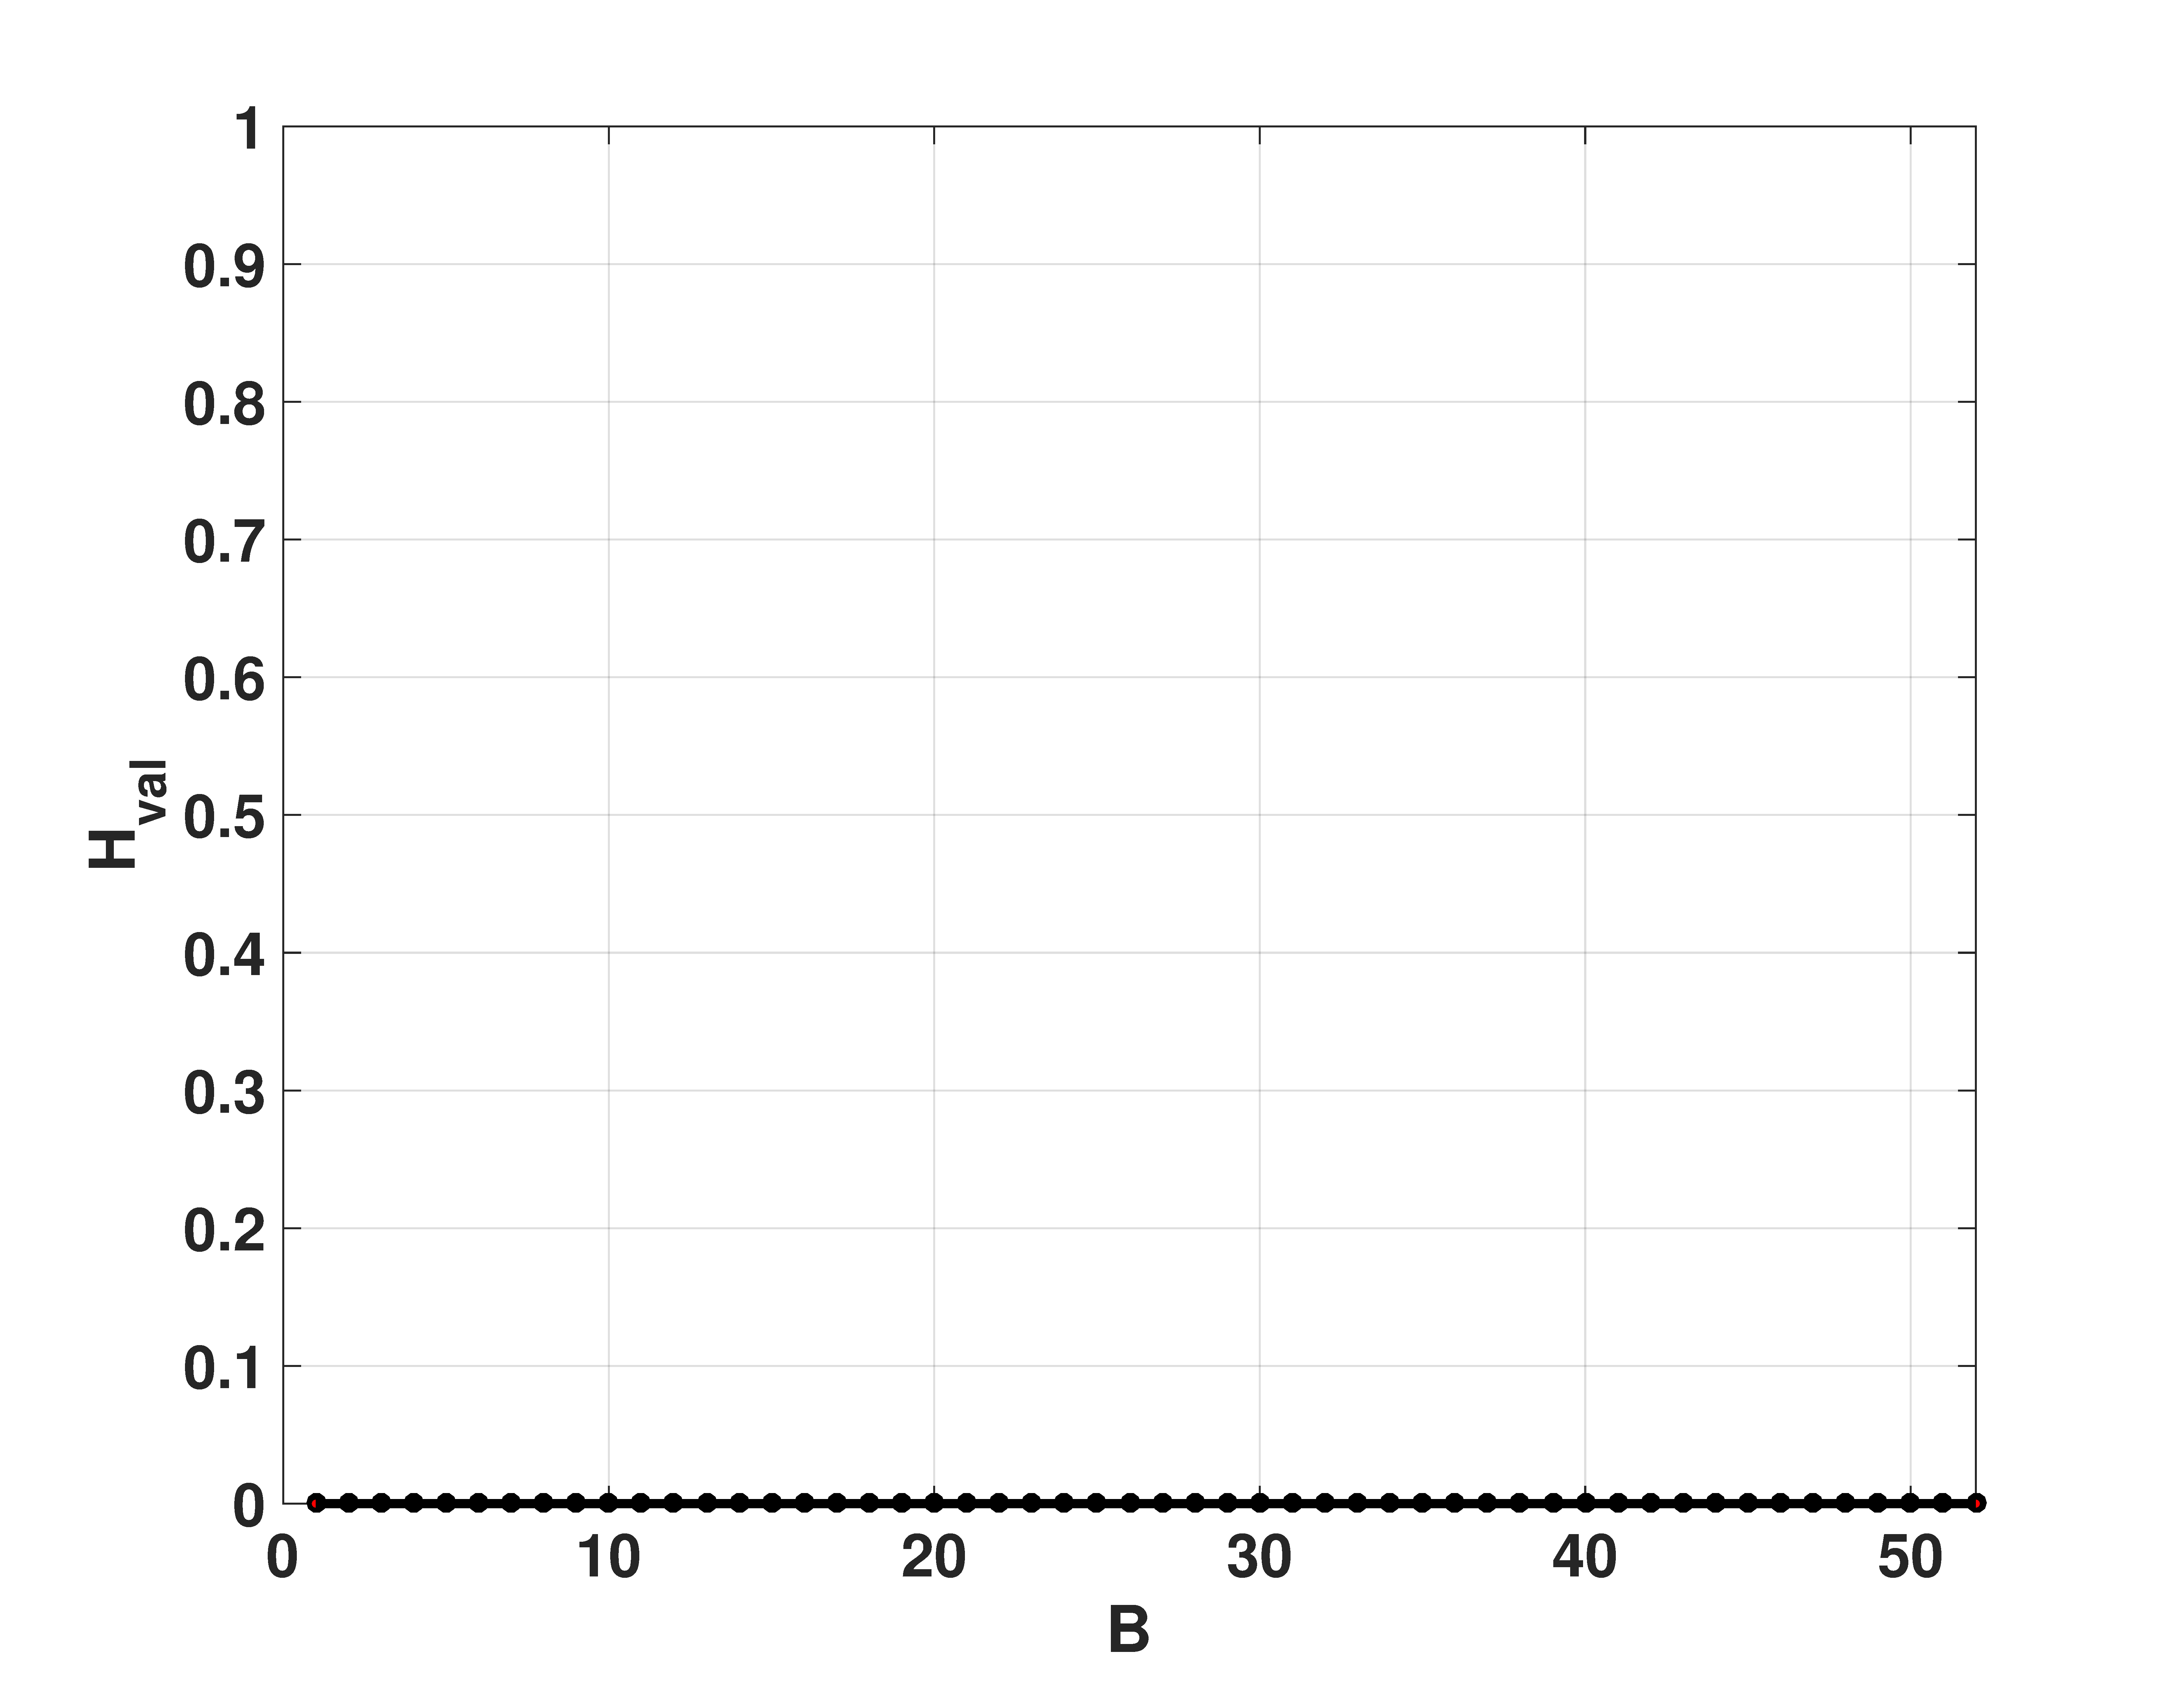
\includegraphics[width=.49\textwidth]{Hval_Tent}
	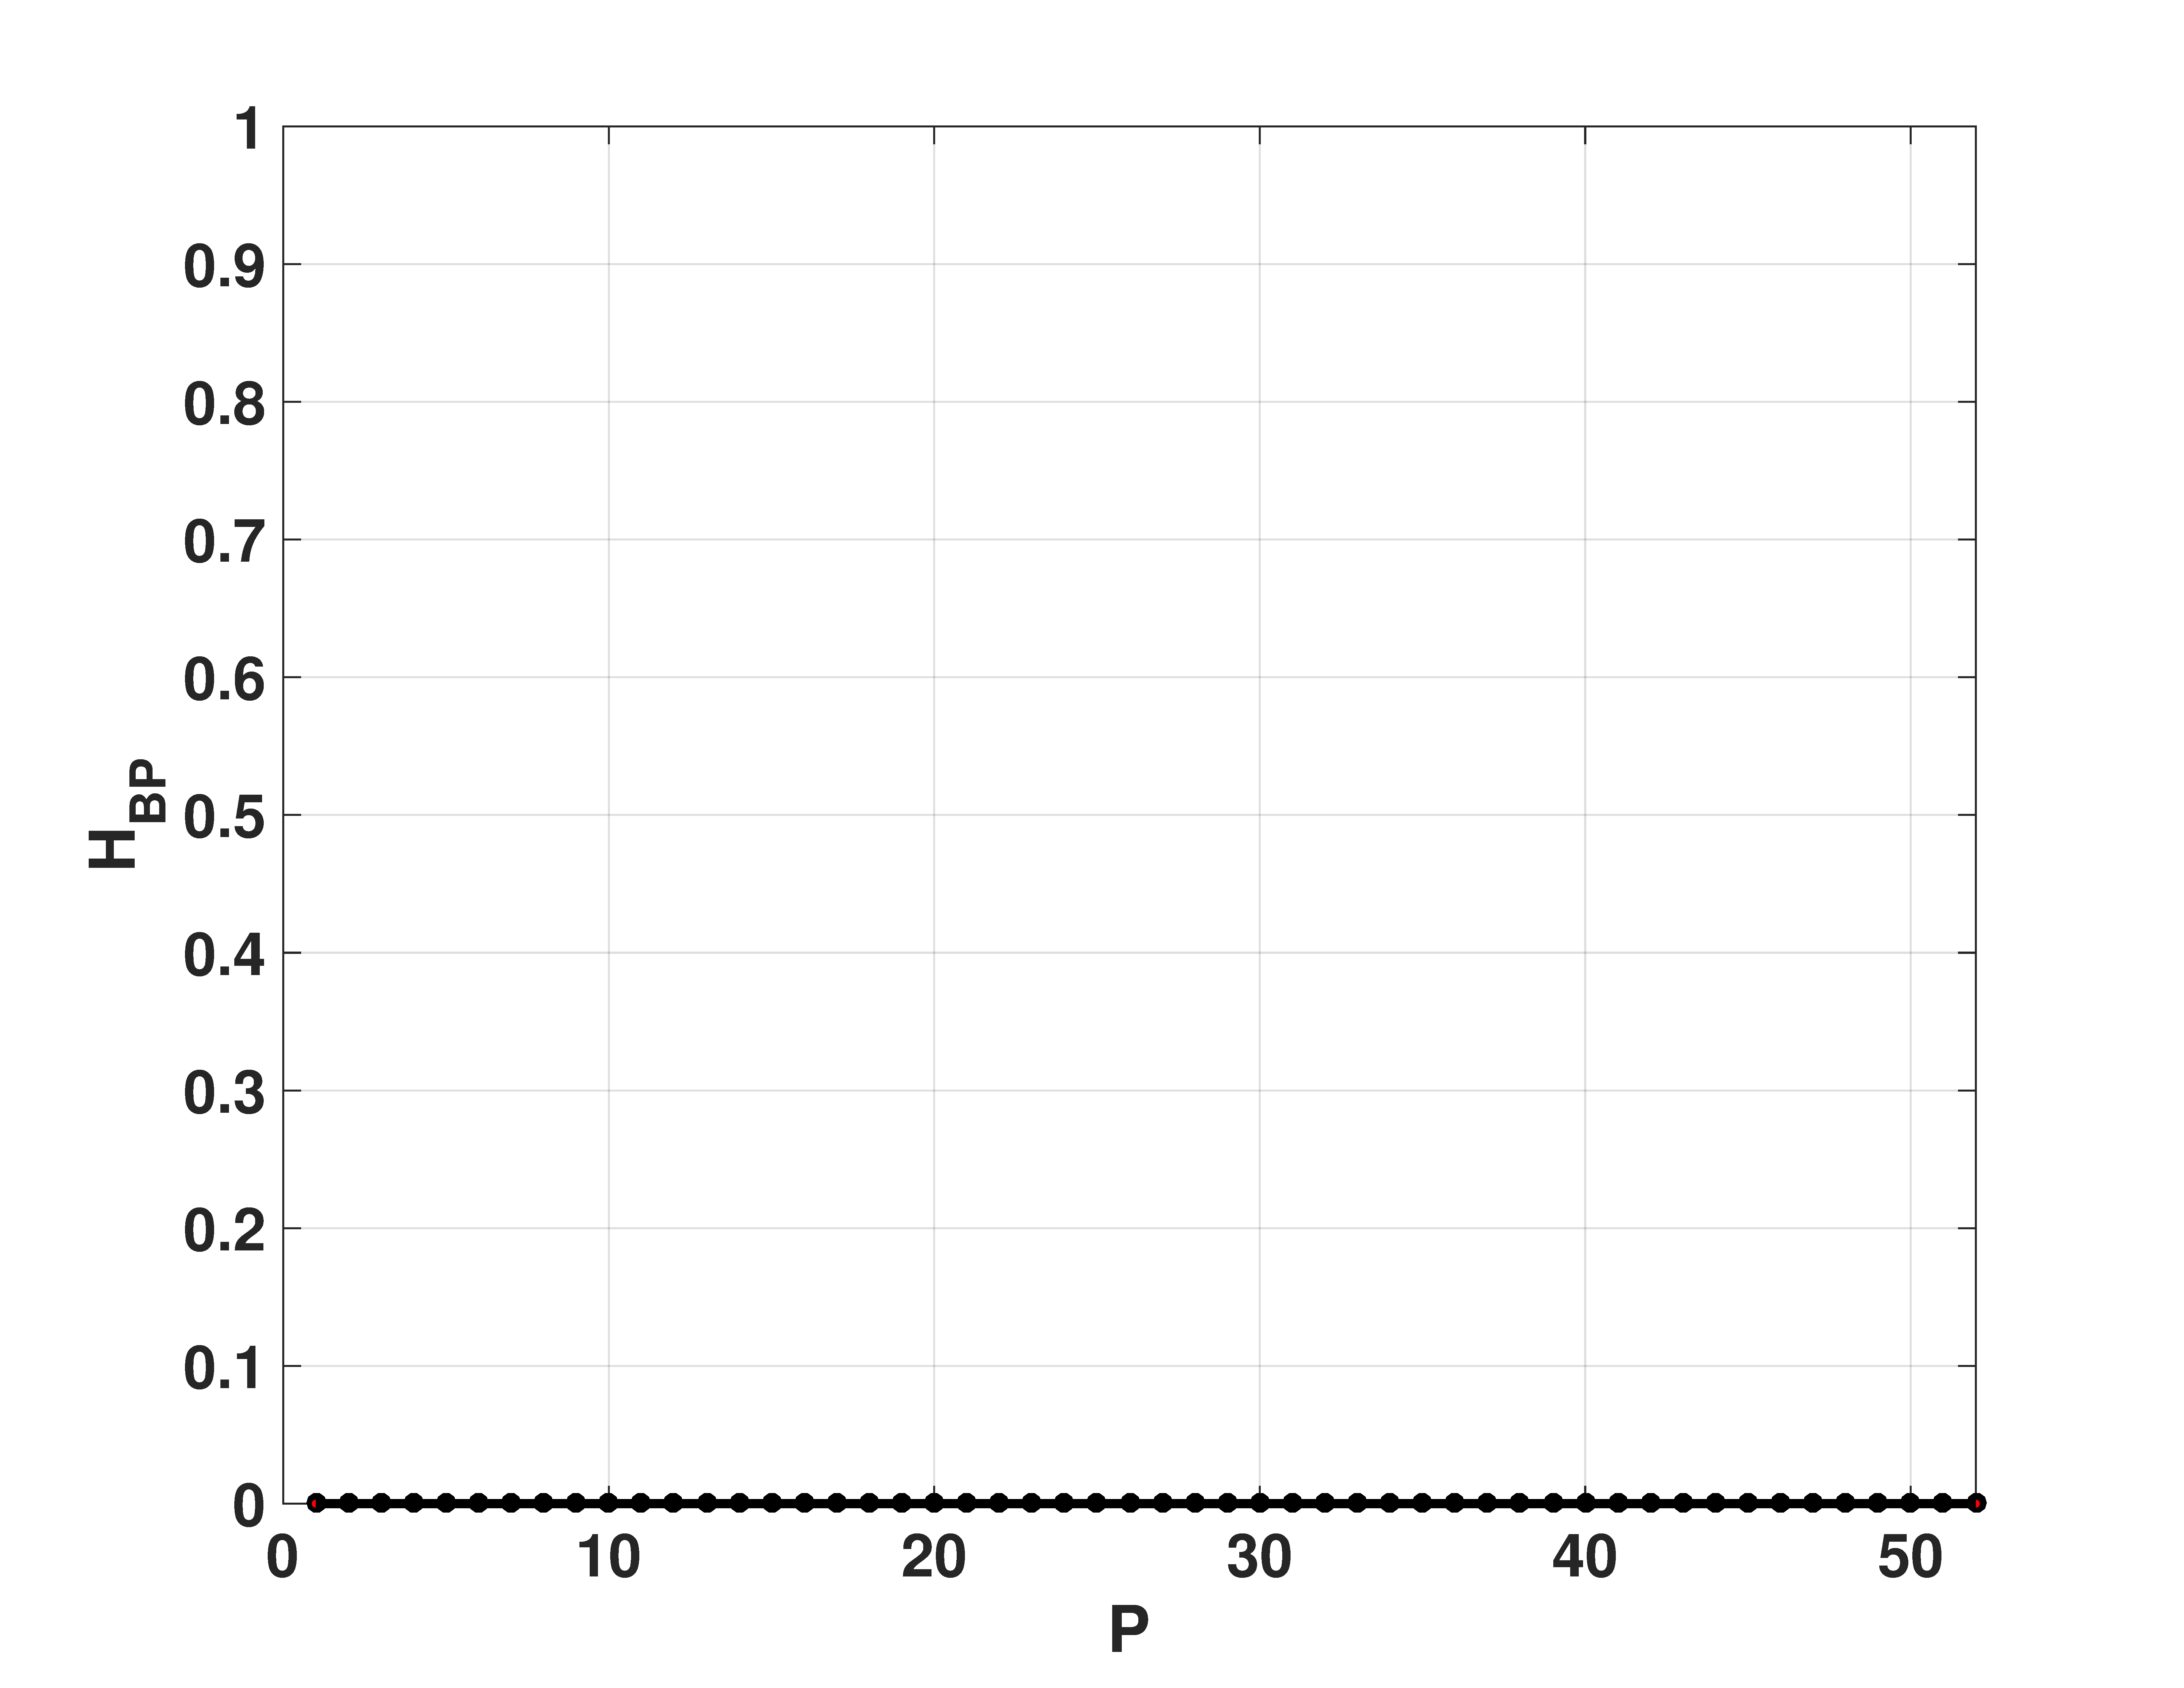
\includegraphics[width=.49\textwidth]{Hbp_Tent}
	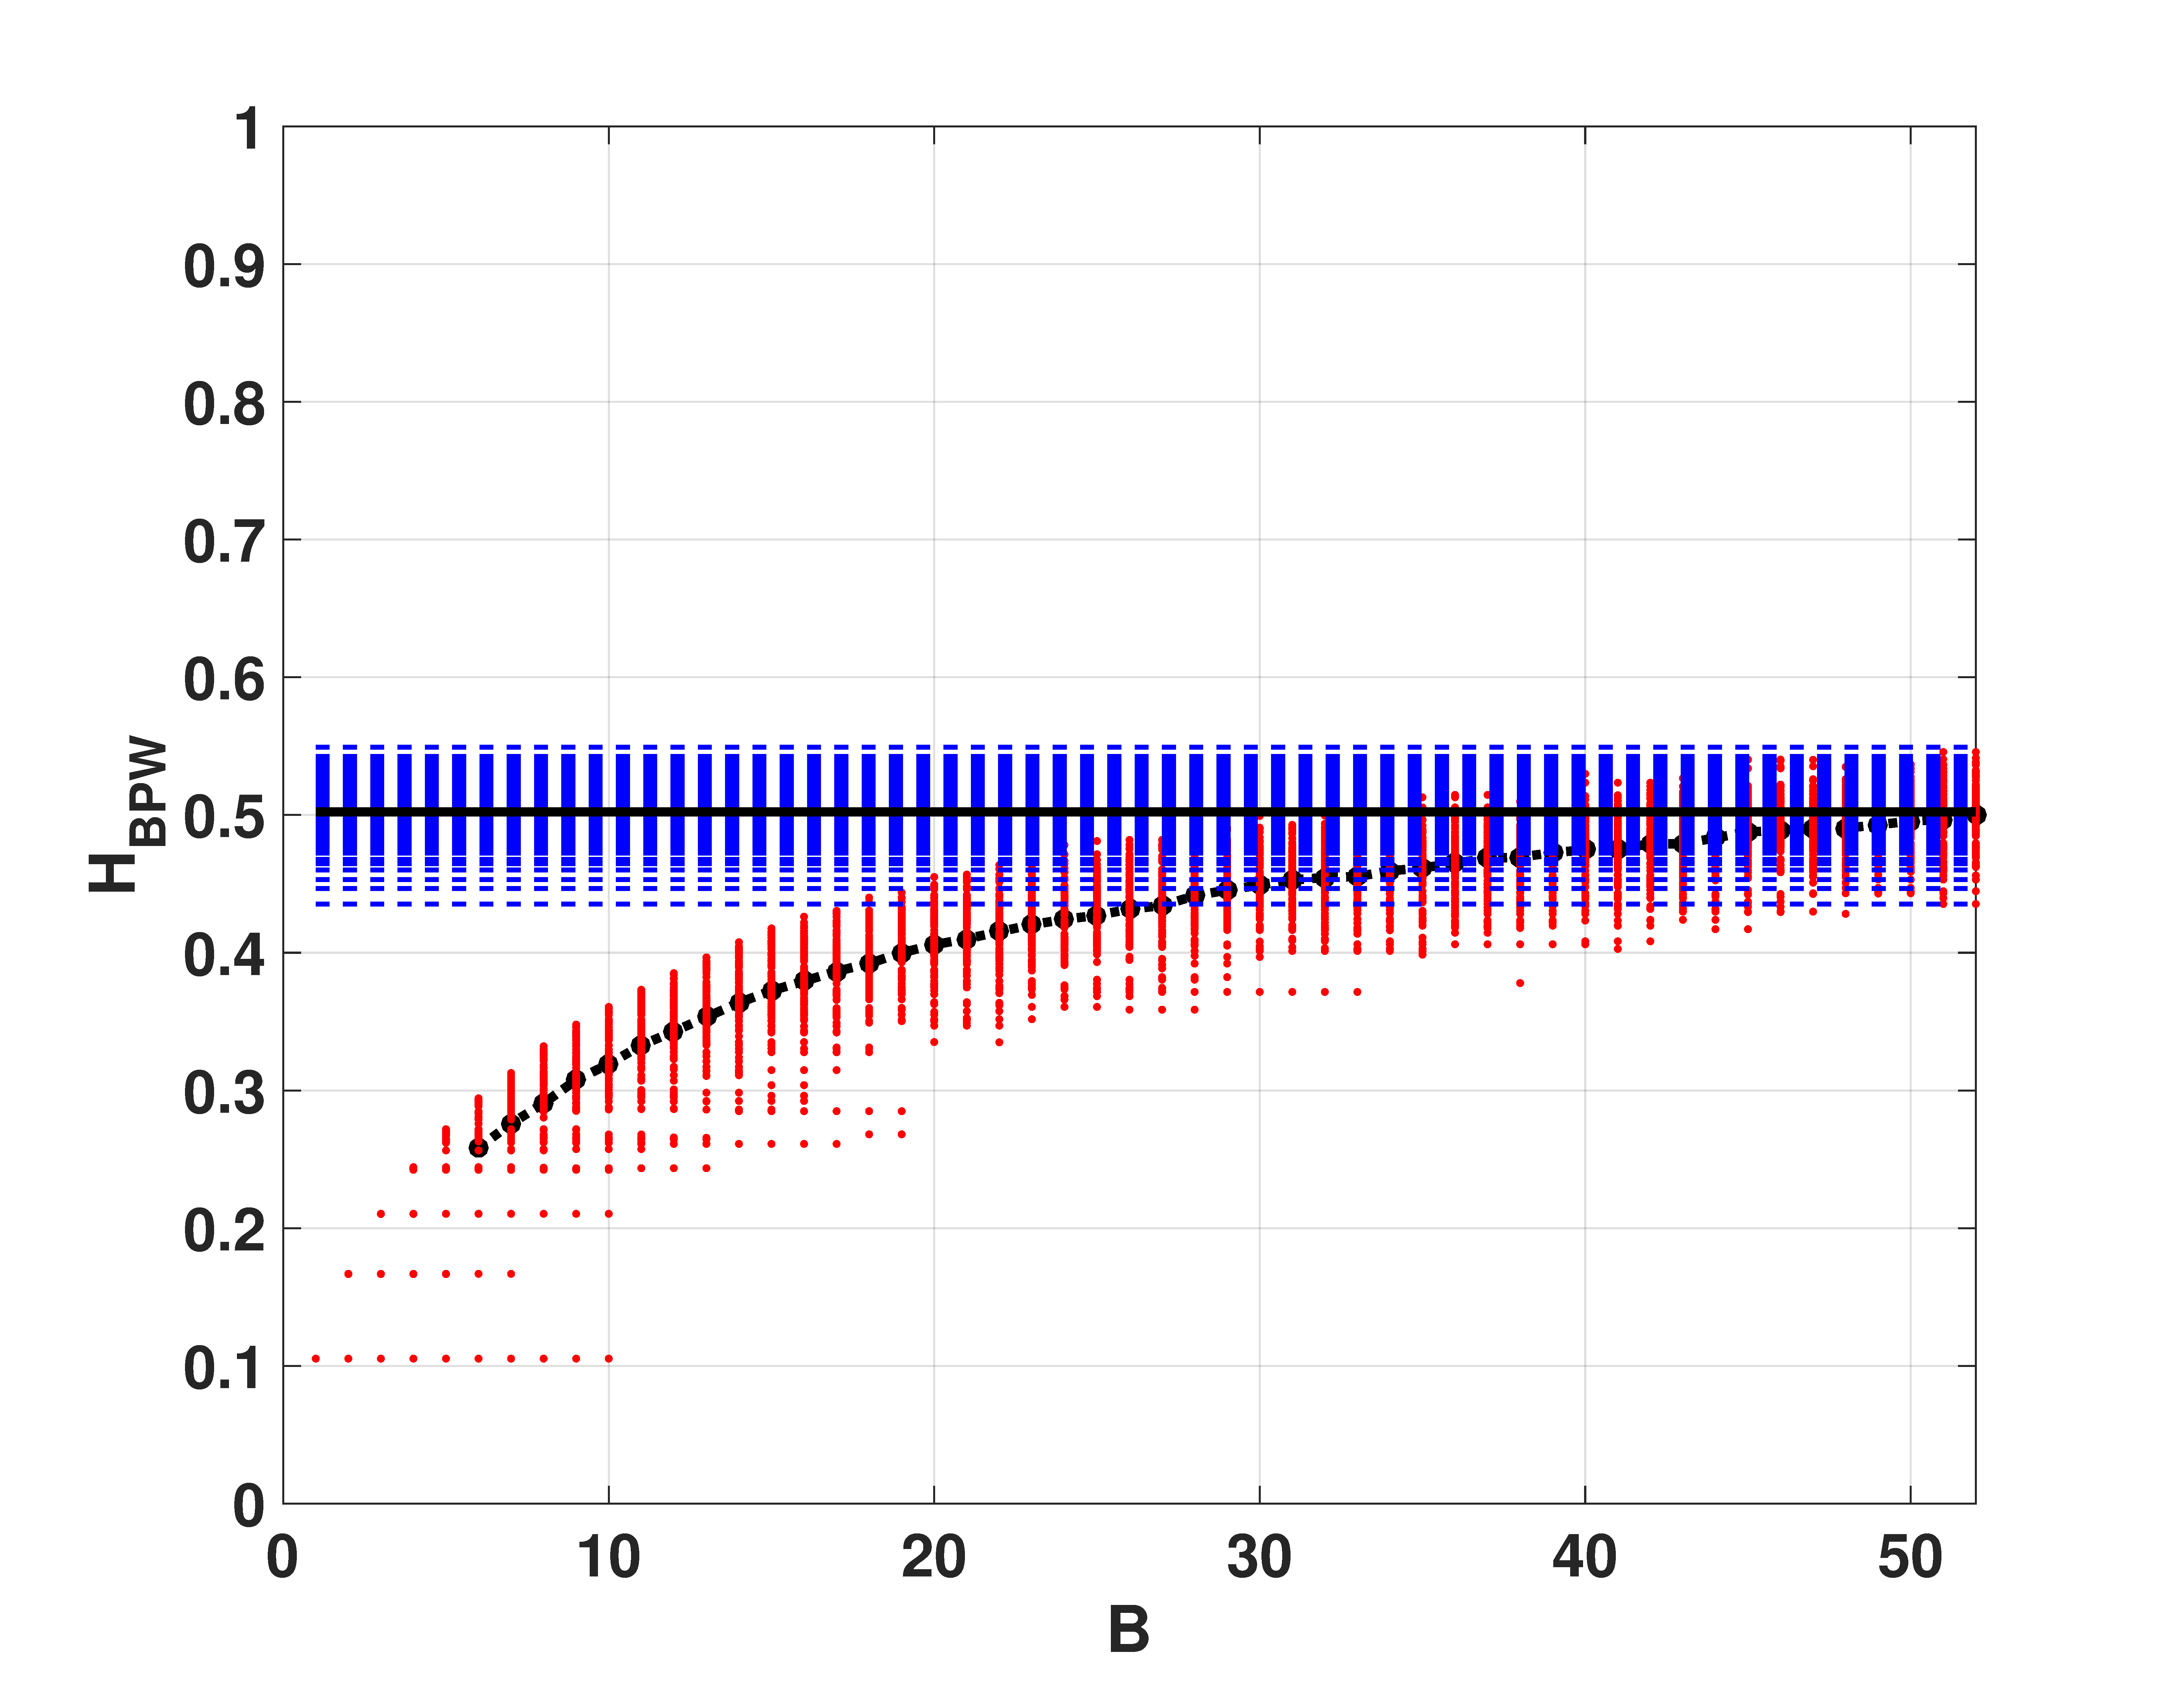
\includegraphics[width=.49\textwidth]{Hbpw_Tent}
	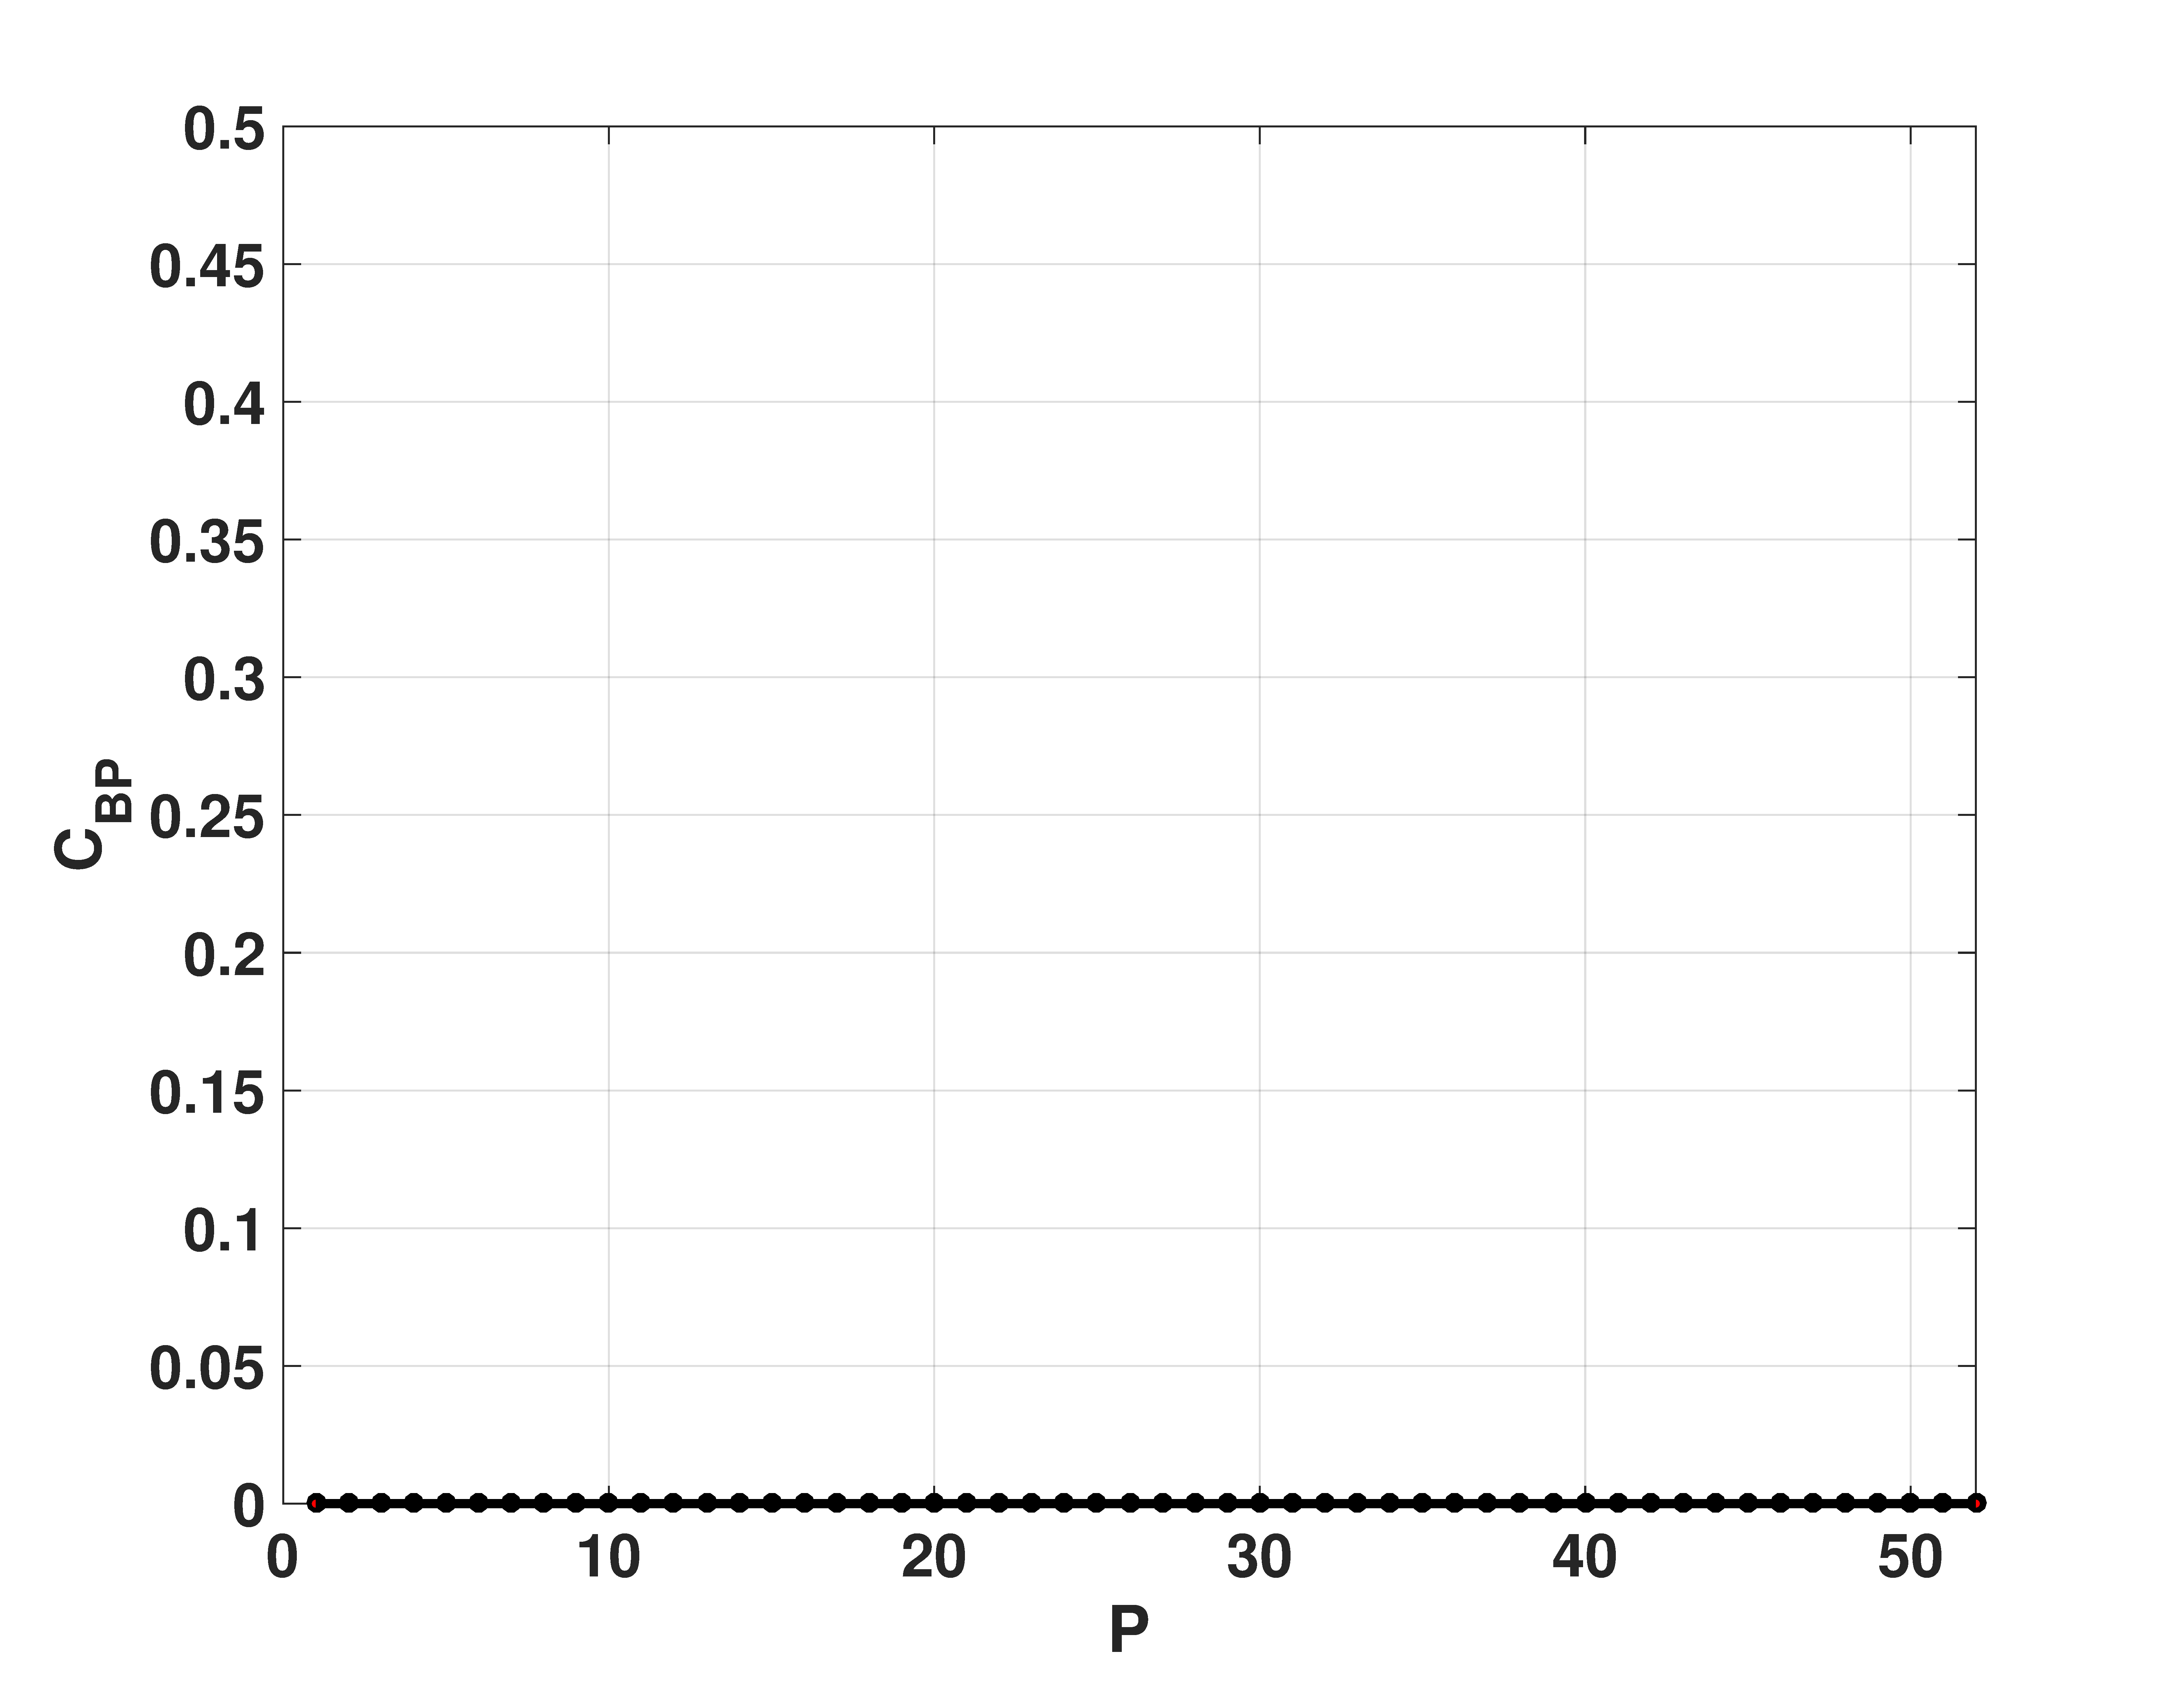
\includegraphics[width=.49\textwidth]{Cbp_Tent}
	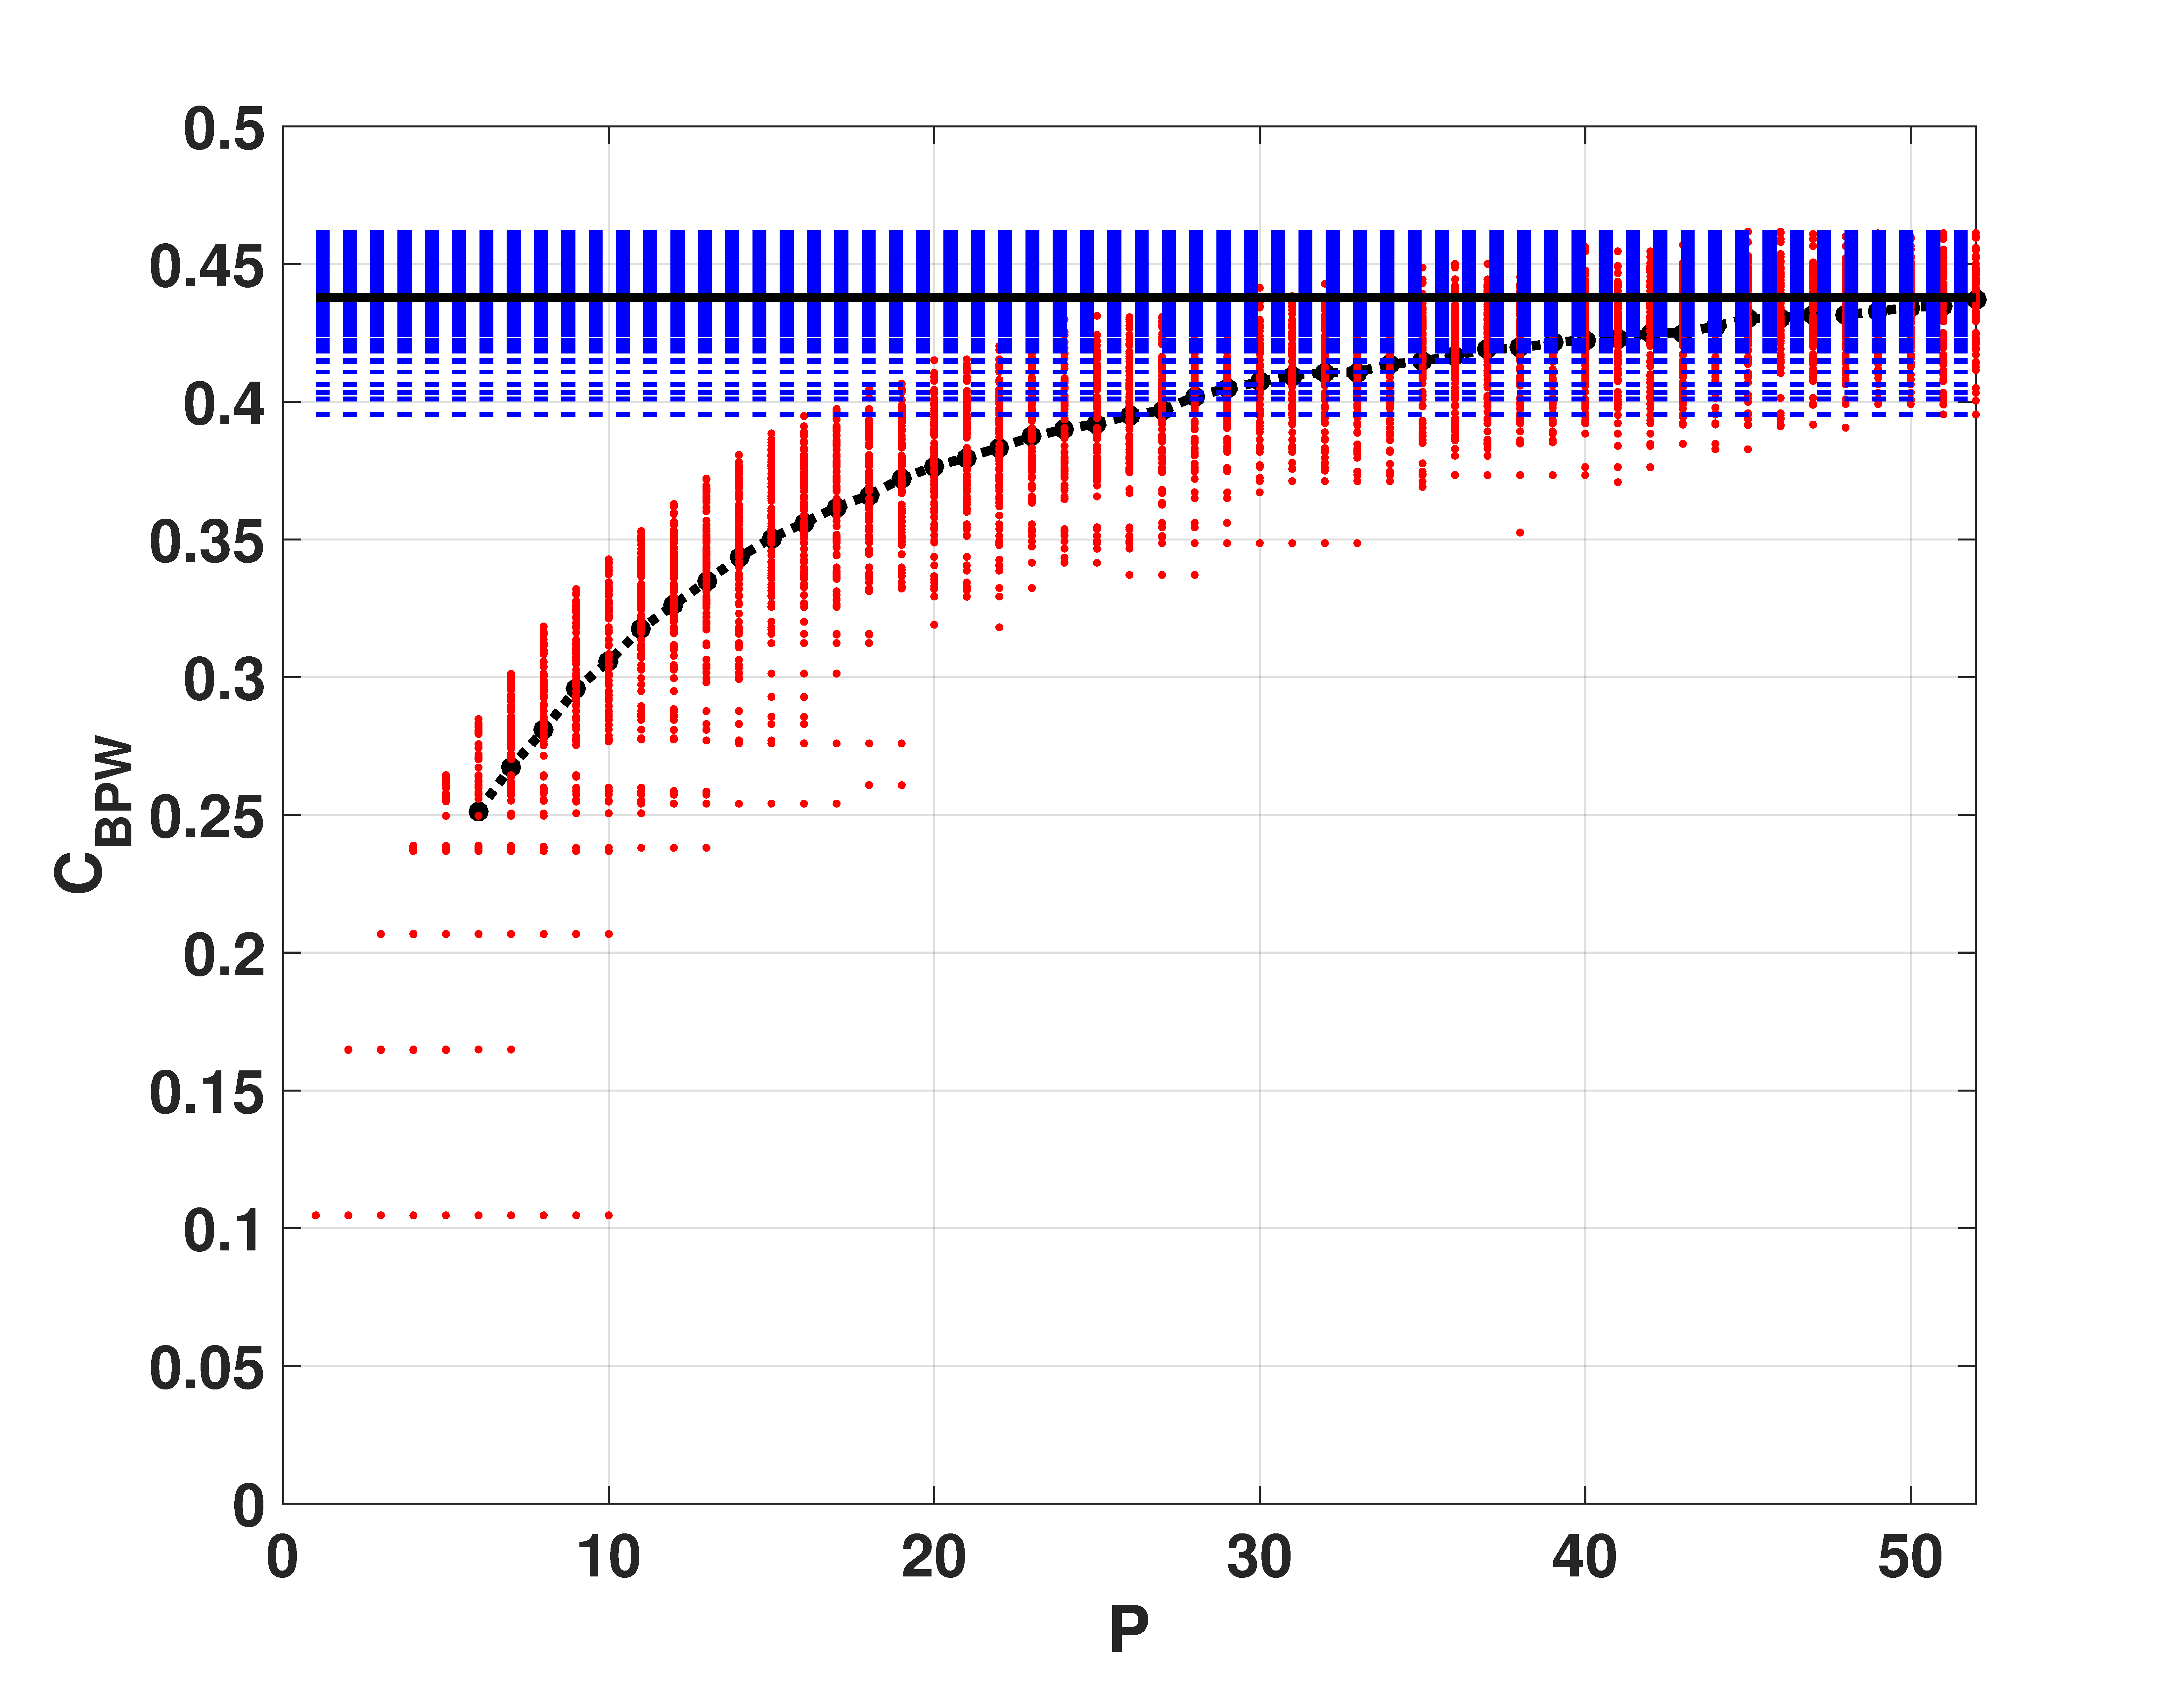
\includegraphics[width=.49\textwidth]{Cbpw_Tent}
	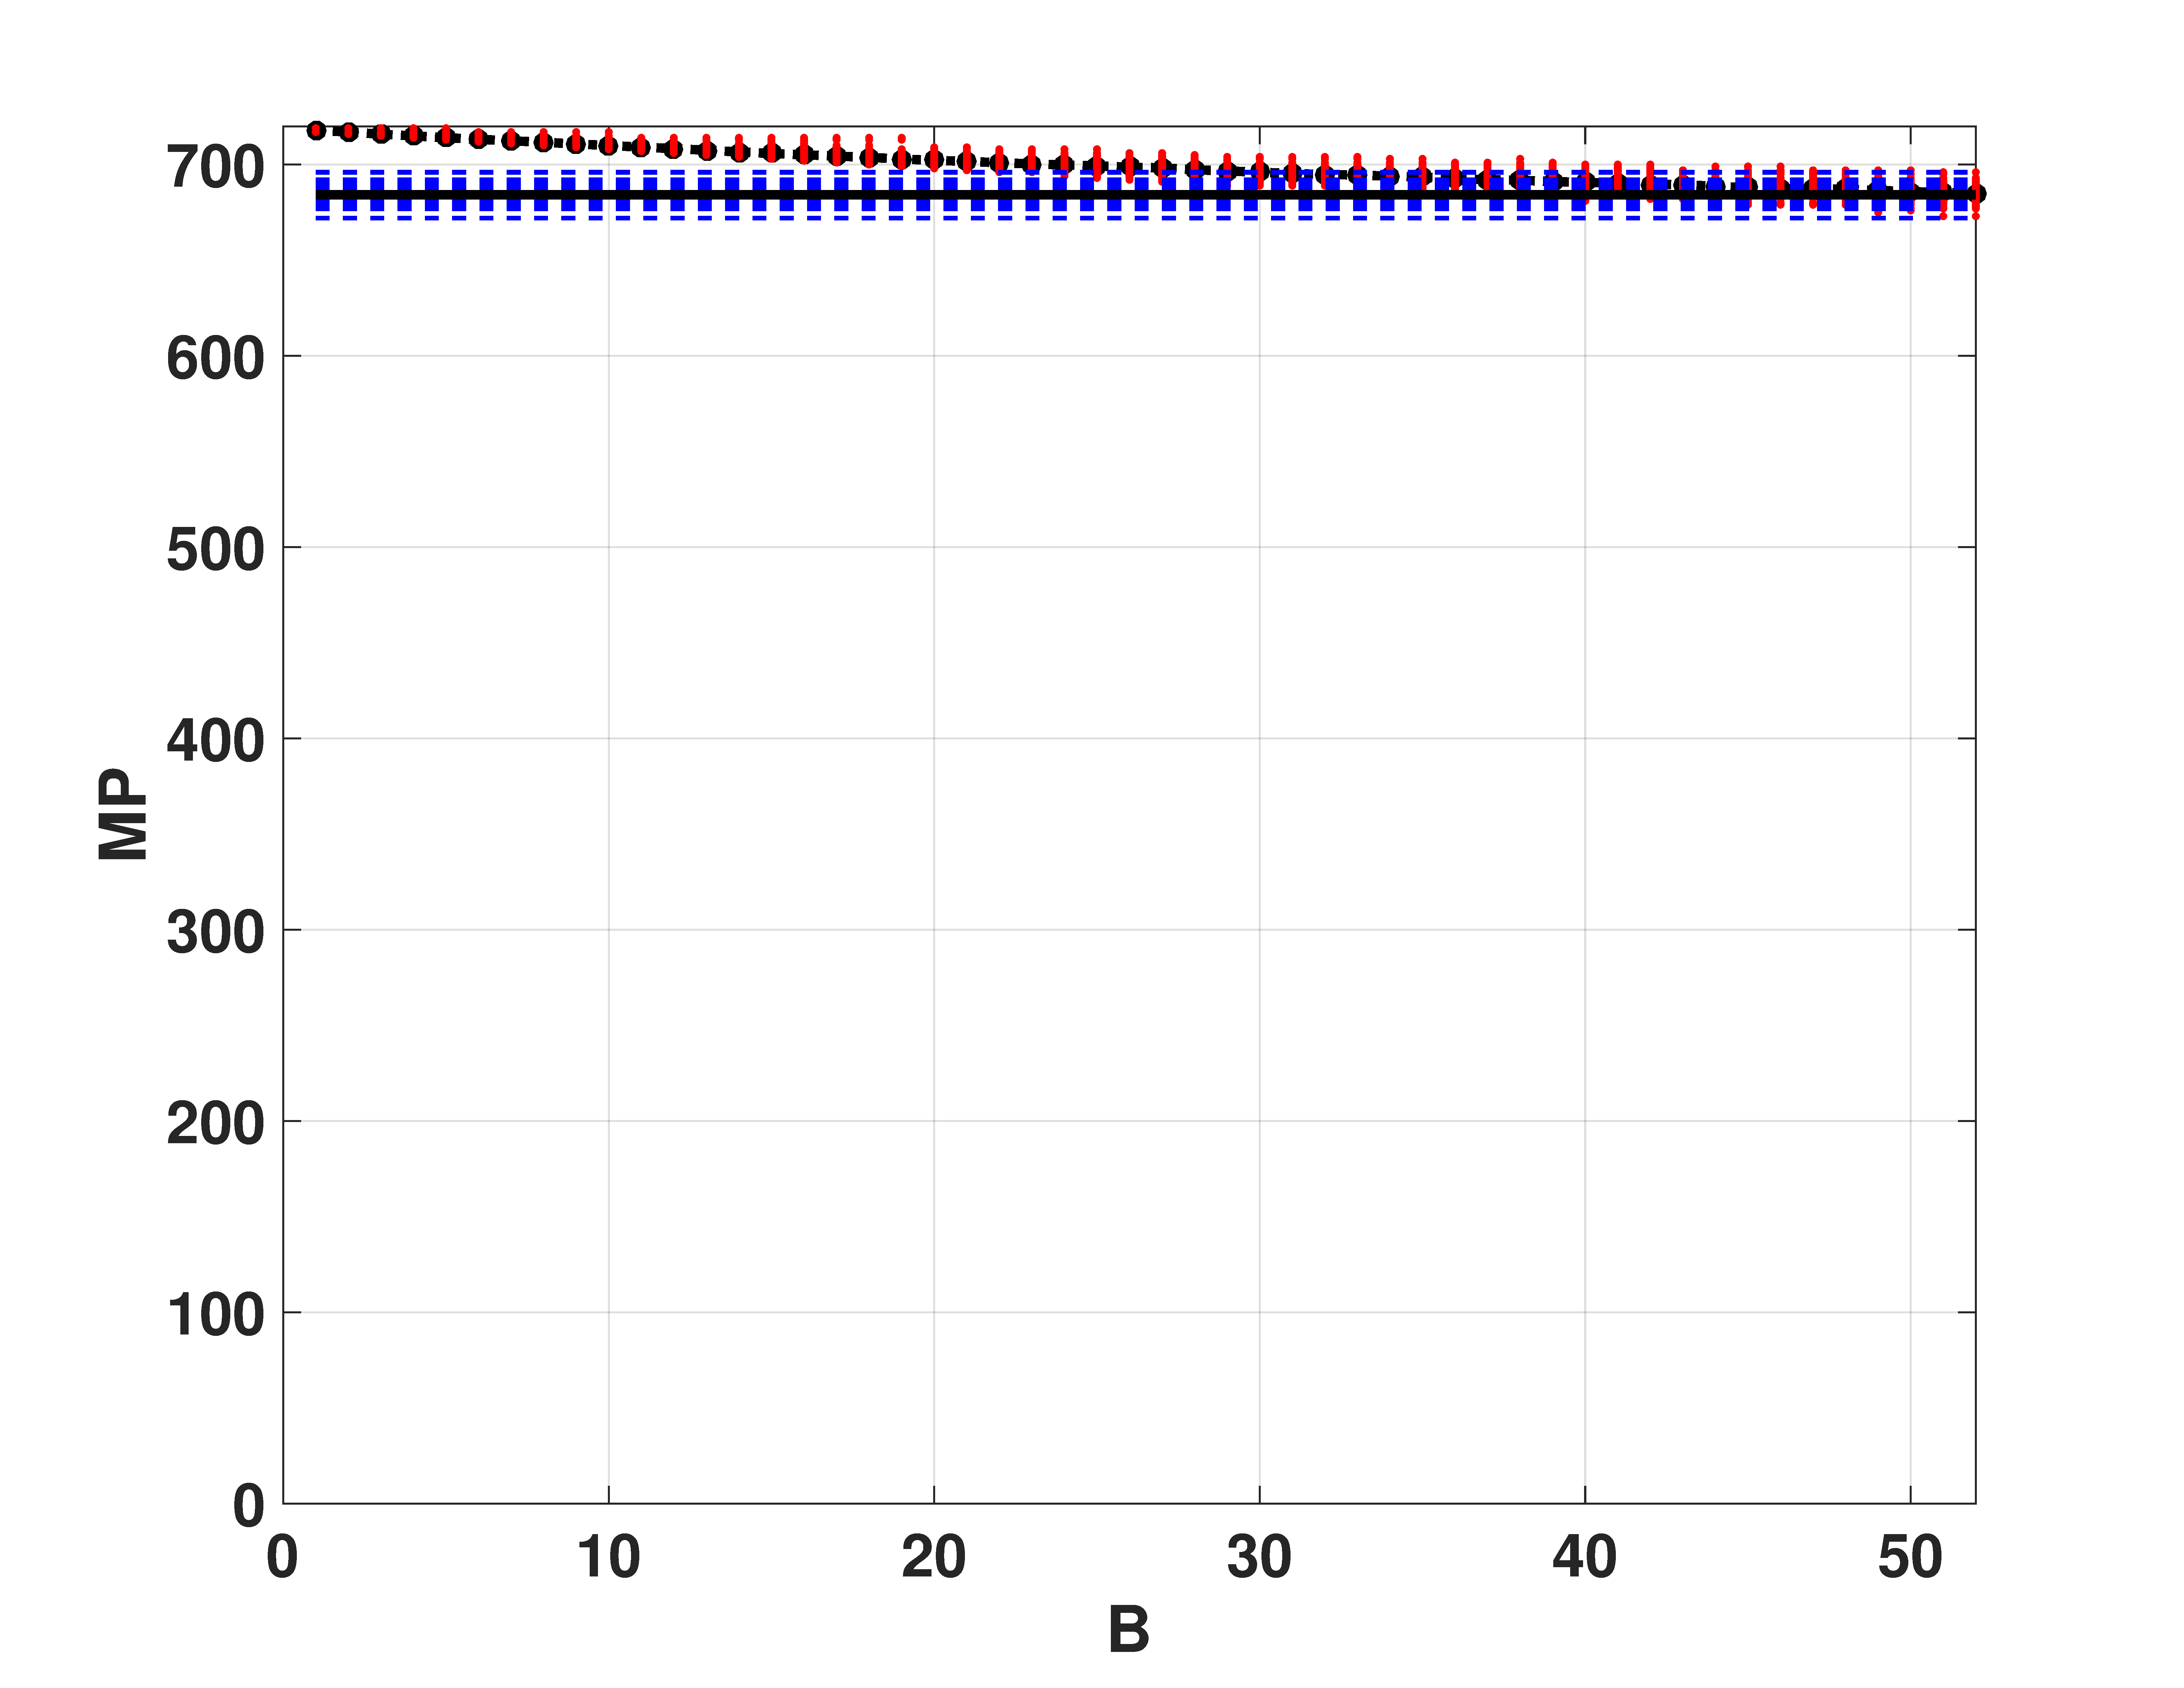
\includegraphics[width=.49\textwidth]{MP_Tent}
	\caption{Statistical properties of the TENT map using binary representation: (a) $H_{val}$ vs $B$ (b) $H_{BP}$ vs $B$ (c) $C_{BP}$ vs $B$ (d) Number of missing ordering patterns $MP$ vs $B$.}
	\label{fig:TENT_QuantiB}
\end{figure}

When fixed point is discarded, complexity remains near maximum for all presicions.
It can be seen in Fig. \ref{fig:TENT_HC}, where all points are close to upper margin.

\begin{figure}
	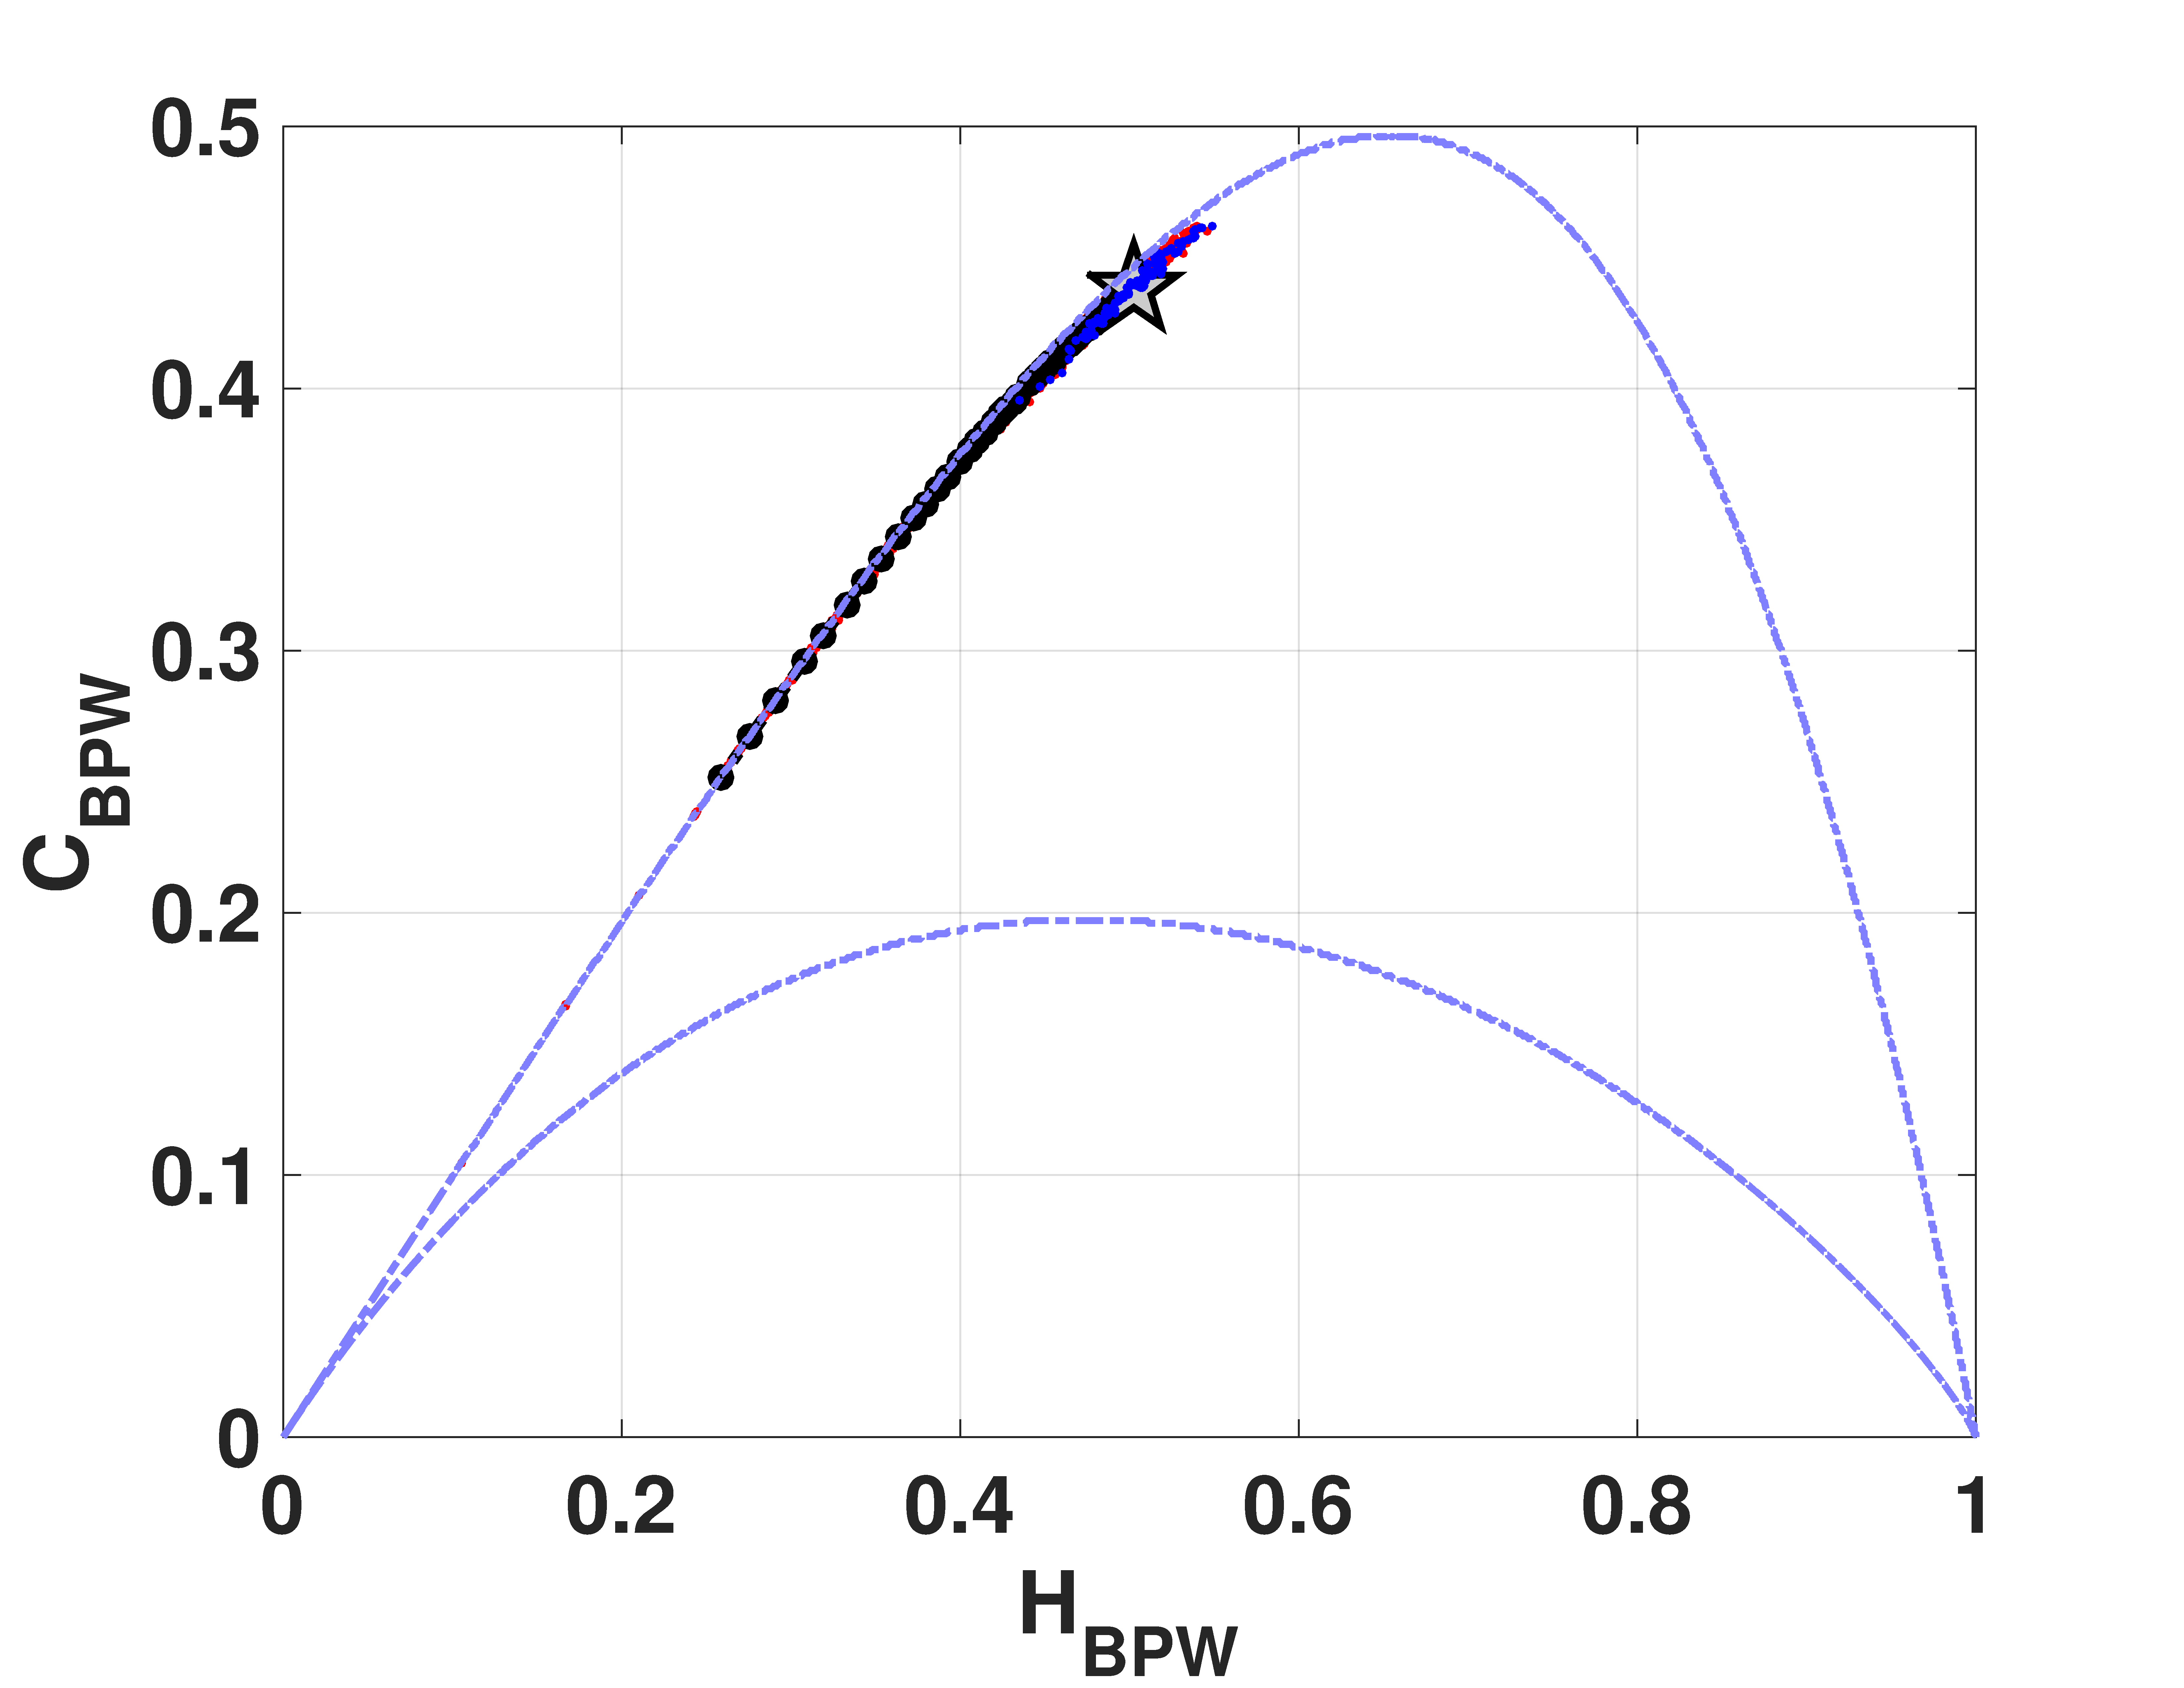
\includegraphics[width=.49\textwidth]{CbpwHbpw_Tent}
	\caption{Evolution of statistical properties in entropy-complexity plane of LOG map using binary representation: $C_{BPW}$ vs $H_{BPW}$.}
	\label{fig:TENT_HC}
\end{figure}
